\section{Solving problems using the semi-implicit models}
\label{tutorial-decoupled}

In contrast to the last section, we now apply a semi-implicit solution procedure, a
so-called \textit{IMPET} (\textit{IM}plicit \textit{P}ressure \textit{E}xplicit 
\textit{T}ransport) algorithm. This means that the pressure equation is first 
solved using an implicit method. The resulting velocities are then used to solve
a transport equation explicitly.\\
In this tutorial, pure fluid phases are solved with a finite volume discretization
of both pressure- and transport step. Primary variables, according to default
settings of the model, are the pressure and the saturation of the wetting phase.

The problem which is solved in this tutorial is the same as for the previous tutorial and is illustrated in figure 
\ref{tutorial-decoupled:problemfigure}: A rectangular domain with no flow 
boundaries on the top and at the bottom, which is initially saturated with oil, 
is considered. Water infiltrates from the left side into the domain. Gravity 
effects are neglected.

\begin{figure}[ht]
\psfrag{x}{x}
\psfrag{y}{y}
\psfrag{no flow}{no flow}
\psfrag{water}{\textbf{water}}
\psfrag{oil}{\textcolor{white}{\textbf{oil}}}
\psfrag{p_w = 2 x 10^5 [Pa]}{$p_w = 2 \times 10^5$ [Pa]}
\psfrag{p_w_initial = 2 x 10^5 [Pa]}{\textcolor{white}{\textbf{$\mathbf{p_{w_{initial}} = 2 \times 10^5}$ [Pa]}}}
\psfrag{S_n = 0}{$S_w = 1$}
\psfrag{S_n_initial = 0}{\textcolor{white}{$\mathbf{S_{w_{initial}} = 0}$}}
\psfrag{q_w = 0 [kg/m^2s]}{$q_w = 0$ $\left[\frac{\textnormal{kg}}{\textnormal{m}^2 \textnormal{s}}\right]$}
\psfrag{q_n = -3 x 10^-4 [kg/m^2s]}{$q_n = 3 \times 10^-2$ $\left[\frac{\textnormal{kg}}{\textnormal{m}^2 \textnormal{s}}\right]$}
\centering
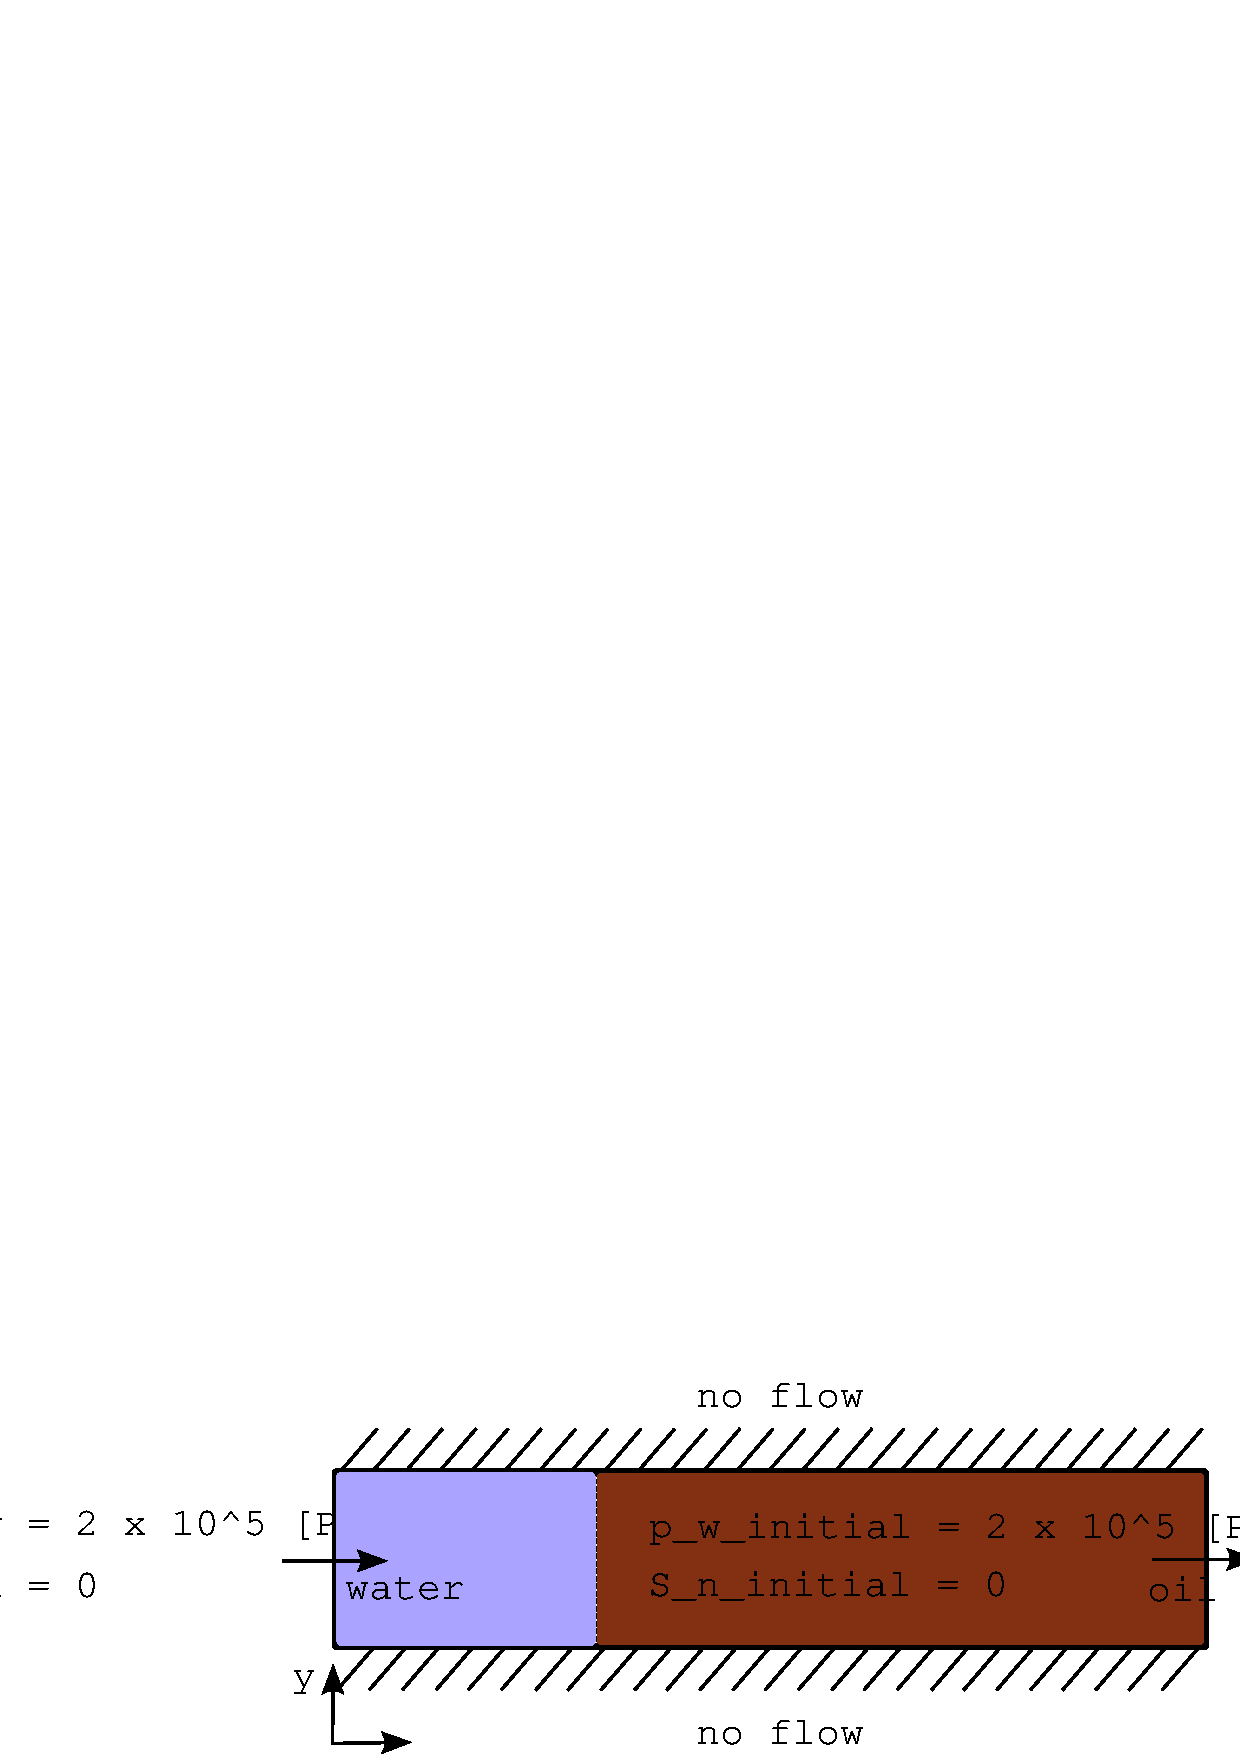
\includegraphics[width=0.9\linewidth,keepaspectratio]{EPS/tutorial-problemconfiguration}
\caption{Geometry of the tutorial problem with initial and boundary conditions.}\label{tutorial-decoupled:problemfigure}
\end{figure}

Listing \ref{tutorial-decoupled:mainfile} shows how the main file, which has to be executed, has to be set up, if the problem described above is to be solved using a semi-implicit model. This main file can be found in the directory \texttt{/tutorial} below the \eWoms base directory.

\begin{lst}[File tutorial/tutorial\_decoupled.cc]\label{tutorial-decoupled:mainfile} \mbox{}
\lstinputlisting[style=eWomsCode, numbersep=5pt, firstline=26, firstnumber=26]{../../tutorial/tutorial_decoupled.cc}
\end{lst}

First, from line \ref{tutorial-decoupled:include-begin} to line
\ref{tutorial-decoupled:include-end} the \Dune and \eWoms files containing
essential functions and classes are included.

At line \ref{tutorial-decoupled:set-type-tag} the type tag of the
problem which is going to be simulated is set. All other data types
can be retrieved by the \eWoms property system and only depend on this
single type tag. For an introduction to the
property system, see section \ref{sec:propertysystem}.

After this, \eWoms' default startup routine \texttt{Ewoms::start()} is
called in line \ref{tutorial-decoupled:call-start}. This function deals
with parsing the command line arguments, 
setting up the infrastructure necessary for \Dune, loading the grid, and
starting the simulation. All parameters can
be either specified by command line arguments of the form
(\texttt{--ParameterName=ParameterValue}), or in the file specified by the
\texttt{--ParameterFile=filename.ini} argument. If a parameter is
specified on the command line as well as in the parameter file, the
values provided in the command line takes
precedence.

\subsection{The problem class} \label{decoupled_problem}

When solving a problem using \eWoms, the most important file is the
so-called \textit{problem file} as shown in listing
\ref{tutorial-decoupled:problemfile} of
\texttt{tutorialproblem\_decoupled.hh}.

\begin{lst}[File tutorial/tutorialproblem\_decoupled.hh]\label{tutorial-decoupled:problemfile} \mbox{}
\lstinputlisting[style=eWomsCode, numbersep=5pt, firstline=27, firstnumber=27]{../../tutorial/tutorialproblem_decoupled.hh}
\end{lst}

First, both \Dune  grid handlers and the semi-implicit model of \eWoms 
have to be included. Then, a new type tag is created for the problem 
in line \ref{tutorial-decoupled:create-type-tag}.  In this case, the 
new type tag inherits all properties defined for the \texttt{DecoupledTwoP} 
type tag, which means that for this problem the two-phase decoupled approach
is chosen as discretization scheme (defined via the include in line 
\ref{tutorial-decoupled:parent-problem}). On line \ref{tutorial-decoupled:set-problem}, 
a problem class is attached to the new type tag, while the grid which
is going to be used is defined in line \ref{tutorial-decoupled:set-grid-type} --
in this case an \texttt{YaspGrid} is created. Since there's no uniform mechanism to
allocate grids in \Dune, \eWoms features the concept of grid creators.
In this case the generic \texttt{CubeGridCreator} (line \ref{tutorial-decoupled:set-gridcreator}) which creates a
structured hexahedron grid of a specified size and resolution. For
this grid creator the  physical domain of the grid is specified via the
run-time parameters \texttt{DomanSizeX},
\texttt{DomanSizeY}, \texttt{CellsX} and
\texttt{CellsY}. These parameters can be specified via
the command-line or in a parameter file.
For more information about the \Dune grid interface, the different grid types 
that are supported and the generation of different grids consult 
the \textit{Dune Grid Interface HOWTO} \cite{DUNE-HP}. 

Next, we select the material of the simulation: In the case of a pure two-phase
model, each phase is a bulk fluid, and the complex (compositional) fluidsystems
do not need to be used. However, they can be used (see exercise 1e). 
Instead, we use a simplified fluidsystem that wraps pure component classes 
for the liquid and gas phases. This is done from line \ref{tutorial-decoupled:2p-system-start} to 
\ref{tutorial-decoupled:2p-system-end}. These components represent fluids made of pure 
chemical species, but given the fact, that a even pure chemical species can assume two phases, only their respective liquid phase is selected on lines \ref{tutorial-decoupled:wettingPhase} and 
\ref{tutorial-decoupled:nonwettingPhase}. For all parameters that depend 
on space, such as the properties of the soil, the specific spatial parameters 
for the problem of interest are specified in line
\ref{tutorial-decoupled:set-spatialparameters}. 

Now we arrive at some model parameters of the applied two-phase semi-implicit 
model. First, in line  \ref{tutorial-decoupled:cflflux} a flux function for the evaluation of the CFL-criterion is defined. This is optional as there exists also a default flux function. The choice depends on the problem which has to be solved. For cases which are not advection dominated, the one chosen here is more reasonable.
Line \ref{tutorial-decoupled:cflfactor} assigns the CFL-factor to be used in the
simulation run, which scales the time step size (kind of security factor). The next property, defined on line \ref{tutorial-decoupled:gravity} 
is optional and tells the model to disregard gravity.
Finally, the default dimensions of the size of the physical and temporal
domains are defined on lines
\ref{tutorial-decoupled:domain-defaults-begin} to
\ref{tutorial-decoupled:domain-defaults-end}.

After all necessary properties are defined and 
its \texttt{Properties} namespace is closed in line \ref{tutorial-decoupled:propertysystem-end},
the problem class is defined in line \ref{tutorial-decoupled:def-problem}. 
As its property, the problem class itself is also derived from a parent, 
\texttt{IMPESProblem2P}.

Beside the definition of the boundary and initial conditions, the problem class also provides
general information about the current simulation. First, the name used by for the
resulting VTK output files is defined by the \texttt{name()} method of line
\ref{tutorial-decoupled:name}, and line \ref{tutorial-decoupled:restart} indicates
when and whether restart files are written. As semi-implicit schemes usually feature small 
timesteps, it can be useful to set an output interval larger than 1. The respective function is called in line \ref{tutorial-decoupled:outputinterval}, which gets the output interval as argument.

The following methods all have in common that they may be dependent on space.
Hence, they all have either an \texttt{element} or an \texttt{intersection} as their
function argument: Both are \Dune entities, depending on whether the parameter of the method is defined in an element, such as 
    initial values, or on an intersection, such as a boundary condition. As it may be sufficient to return values only based on a position, \eWoms models can also access functions in the problem with the form \mbox{\texttt{...AtPos(GlobalPosition\& globalPos)}}, without an \Dune entity, as one can see in line \ref{tutorial-decoupled:bctype}.

There are also methods for terms of the partial differential equations which must be provided such as the source term, boundary conditions (lines \ref{tutorial-decoupled:bctype} to
\ref{tutorial-decoupled:neumann}) and initial values for the transported
quantity in line \ref{tutorial-decoupled:initial}. For more information
on the functions, consult the documentation in the code.

\subsection{The definition of the parameters that are dependent on space}\label{tutorial-decoupled:description-spatialParameters}

Listing \ref{tutorial-decoupled:spatialparametersfile} shows the file
\verb+tutorialspatialparams_decoupled.hh+:

\begin{lst}[File tutorial/tutorialspatialparams\_decoupled.hh]\label{tutorial-decoupled:spatialparametersfile} \mbox{}
\lstinputlisting[style=eWomsCode, numbersep=5pt, firstline=27, firstnumber=27]{../../tutorial/tutorialspatialparams_decoupled.hh}
\end{lst}
The argument list for its methods here is the same as for the problem 
functions: Either an \texttt{element}, or only the global position if the function is called \texttt{...AtPos(...)}.

\subsection{Exercises}
\label{tutorial-deoucpled:exercises}
The following exercises will give you the opportunity to learn how you
can change soil parameters, boundary conditions and fluid properties
in \eWoms and is intended to give you an opportunity to play with the
semi-implicit modelling framework.

\subsubsection{Exercise 1}
\renewcommand{\labelenumi}{\alph{enumi})}
For Exercise 1 you only have to make some small changes in the tutorial files.
\begin{enumerate}
\item \textbf{Altering output}

  To get an impression what the results should look like, you can run
  the unmodified version of the semi-implicit tutorial problem by
  typing \texttt{./tutorial\_decoupled}. The runtime parameters which
  are set printed at the start of the simulation. You may either
  specify values for them on the command line by passing the program
  \texttt{--ParameterName=Value} arguments, or by putting parameters
  into a filie and instructing the program to load it by adding the
  command line option \texttt{--ParameterFile=filename}. For a
  description of the available parameters options you add the
  \texttt{--help} command line argument to the program. For the
  visualizing the output using paraview please refer to
  \ref{quick-start-guide}.

  As you can see, the simulation creates many output files. To reduce
  these in order to perform longer simulations, change the method
  responsible for output (line \ref{tutorial-decoupled:outputinterval}
  in the file \texttt{tutorialproblem\_decoupled}) so that it only
  writes an output file every 20 time steps. Re-compile the program by
  typing \texttt{make tutorial\_decoupled} and run it again. Now, run
  the simulation for $500\;000$ seconds.

\item \textbf{Changing the Model Domain} \\
Change the size of the model domain so that you get a rectangle
with edge lengths of x = 300 m \\  and y = 300 m and with discretisation lengths of  $\Delta \text{x} = 20$ m and $\Delta \text{y} = 10$ m. \\


\item \textbf{Changing the Boundary Conditions} \\
Change the boundary conditions in the file \texttt{tutorialproblem\_decoupled.hh} so that water enters from the bottom and oil flows out at the top boundary. The right and the left boundary should be closed for water and oil fluxes. The Neumannn Boundary conditions are multiplied by the normal (pointing outwards), so an influx is negative, an outflux always positive. Such information can easily be found in the documentation of the functions (also look into base classes).

\item \textbf{Changing Fluids} \\
Now change the fluids: Use DNAPL instead of LNAPL and brine instead of water. To do that you have to select different components:
\begin{enumerate}
 \item Brine: First, you need to add an \texttt{\#include} directive for \texttt{brine.hh}. The class \texttt{Ewoms::Brine} is an adapter class that slightly adapts the thermodynamic properties of pure water by adding some salt. Hence, the class \texttt{Ewoms::Brine} uses a pure water class, such as \texttt{Ewoms::H2O}, as a second template argument after the data type \texttt{<Scalar>} as a template argument.
 \item DNAPL: First, you need to change \texttt{\#include} directive from \texttt{lnapl.hh} to \texttt{dnapl.hh}. Then change the fluid used for the non-wetting phase from \texttt{LNAPL<Scalar>} to \texttt{DNAPL<Scalar>}
\end{enumerate}
If you want to take a closer look at how the fluid classes are defined and which substances are already available you may browse the files in the directory
\texttt{/ewoms/material/components}.

\item \textbf{Use an \eWoms fluid system}\label{dec-ex1-fluidsystem} \\
\eWoms usually organizes fluid mixtures via a \textit{fluid system}, see also chapter \ref{sec:fluidframework}. In order to include a fluid system you first have to comment the lines \ref{tutorial-coupled:2p-system-start} to \ref{tutorial-coupled:2p-system-end} in the problem file.\\

Now include the file \texttt{fluidsystems/h2oairsystem.hh} in the
material folder, and set a property \texttt{FluidSystem} with the
appropriate type,
\texttt{Ewoms::FluidSystems::H2OAir<Scalar>}. However, this rather
complicated fluidsystem uses tabularized fluid data, which need to be
initialized at startup (i.e. the tables need to be filled with values)
in the constructor body of the current problem by adding
\texttt{GET\_PROP\_TYPE(TypeTag, FluidSystem)::init();}. Remember that
the constructor function always has the same name as the respective
class, i.e. \texttt{TutorialProblemDecoupled(..)}.

The density of the gas is magnitudes smaller than that of oil, so it
is advisable to decrease the injection rate to $q_n = -3 \cdot 10^{-4}
\frac{\text{kg}}{\text{m}^2 \text{s}}$. Also reduce the simulation
duration to $20\;000$ seconds.

Before you proceed, please revert the changes made in this exercise,
as we still use bulk phases and hence do not need such an extensive
fluid system.
 
\item \textbf{Heterogeneities}  \\
  Set up a model domain with the soil properties given in Figure
  \ref{tutorial-deoucpled:exercise1_d}. Adjust the boundary conditions
  so that water is again flowing from left to right.
\begin{figure}[ht]
\psfrag{K1 =}{K $= 10^{-8}\text{ m}^2$}
\psfrag{phi1 =}{$\phi = 0.15$}
\psfrag{K2 =}{\textcolor{white}{K $= 10^{-9}\text{ m}^2$}}
\psfrag{phi2 =}{\textcolor{white}{$\phi = 0.3$}}
\psfrag{600 m}{600 m}
\psfrag{300 m}{300 m}
\centering
\includegraphics[width=0.5\linewidth,keepaspectratio]{EPS/exercise1_c.eps}
\caption{Exercise 1d: Set-up of a model domain a heterogeneity. $\Delta \text{x} = 20$ m $\Delta \text{y} = 20$ m.}\label{tutorial-deoucpled:exercise1_d}
\end{figure}
When does the front cross the material border? In paraview, the option \textit{View} $\rightarrow$ \textit{Animation View} is nice to get a rough feeling of the timestep sizes.
\end{enumerate}

\subsubsection{Exercise 2}
For this exercise you should create a new problem file analogous to
the file \texttt{tutorialproblem\_decoupled.hh} (e.g. with the name 
\texttt{ex2\_tutorialproblem\_decoupled.hh} and new spatial parameters 
just like \texttt{tutorialspatialparams\_decoupled.hh}. These files need to
be included in the file \texttt{tutorial\_decoupled.cc}. 

Each new files should contain the definition of a new class with a 
name that relates to the file name, such as \texttt{Ex2TutorialProblemDecoupled}. 
Make sure that you also adjust the guardian
macros in lines \ref{tutorial-decoupled:guardian1} and \ref{tutorial-decoupled:guardian2}
 in the header files (e.g. change \\
\texttt{EWOMS\_TUTORIALPROBLEM\_DECOUPLED\_HH} to
\texttt{EWOMS\_EX2\_TUTORIALPROBLEM\_DECOUPLED\_HH}).  Beside also adjusting the guardian macros, 
the new problem file should define and use a new type tag for the problem as well as a new problem class
e.g. \texttt{Ex2TutorialProblemDecoupled}. Make sure to assign your newly defined spatial 
parameter class to the \texttt{SpatialParams} property for the new 
type tag. 

After this, change the domain size (parameter input file) to match the domain described
by figure \ref{tutorial-decoupled:ex2_Domain}. Adapt the problem class
so that the boundary conditions are consistent with figure
\ref{tutorial-decoupled:ex2_BC}. Initially, the domain is fully saturated
with water and the pressure is $p_w = 2 \cdot 10^5 \text{Pa}$ . Oil
infiltrates from the left side. Create a grid with $20$ cells in
$x$-direction and $10$ cells in $y$-direction. The simulation time
should be set to $2e4 \text{s}$.

Now include your new problem file in the main file and replace the
\texttt{TutorialProblemDecoupled} type tag by the one you've created and
compile the program.


\begin{figure}[ht]
\psfrag{K1}{K $= 10^{-7}\text{ m}^2$}
\psfrag{phi1}{$\phi = 0.2$}
\psfrag{Lin}{Brooks Corey Law} 
\psfrag{Lin2}{$\lambda = 1.8$, $p_b = 100$}
\psfrag{K2}{K $= 10^{-9}\text{ m}^2$}
\psfrag{phi2}{$\phi = 0.15$}
\psfrag{BC1}{Brooks Corey Law} 
\psfrag{BC2}{$\lambda = 2$, $p_b = 500$}
\psfrag{H1y}{50 m}
\psfrag{H2y}{15 m}
\psfrag{H3y}{20 m}
\psfrag{L1x}{100 m}
\psfrag{L2x}{50 m}
\psfrag{L3x}{25 m}
\centering
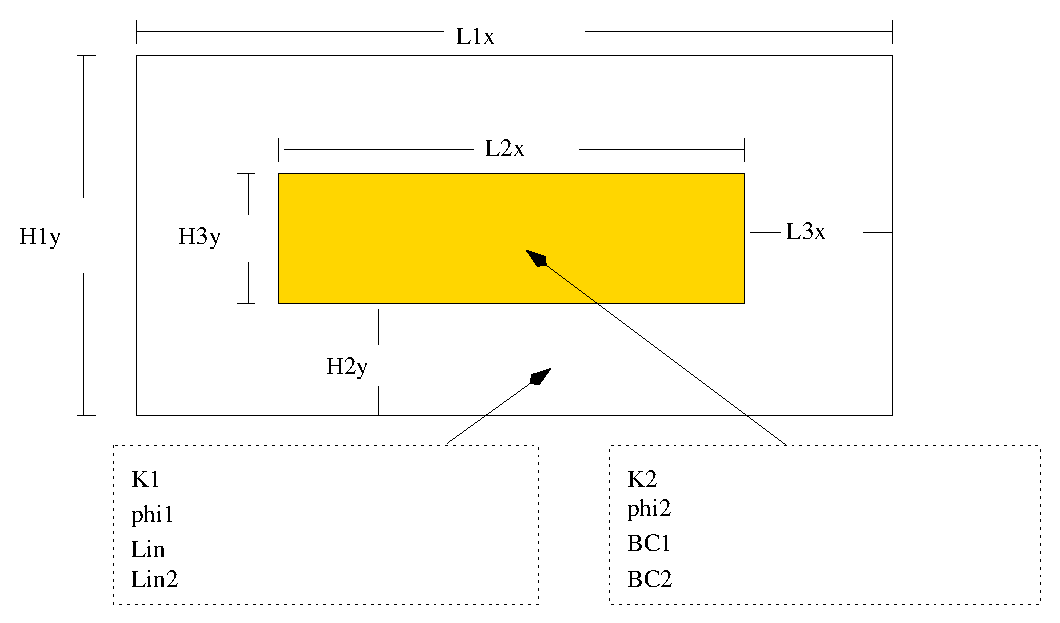
\includegraphics[width=0.8\linewidth,keepaspectratio]{EPS/Ex2_Domain.eps}
\caption{Set-up of the model domain and the soil parameters}\label{tutorial-decoupled:ex2_Domain}
\end{figure}

\begin{figure}[ht]
\psfrag{pw}{$p_w = 2 \times 10^5$ [\text{Pa}]}
\psfrag{S}{$S_w = 0.0$}
\psfrag{qw}{$q_w = 3 \times 10^{-4}$ [kg/$\text{m}^2$s]}
\psfrag{qo}{$q_n = 0.0$ [kg/$\text{m}^2$s]}
\psfrag{no flow}{no flow}
\centering
\includegraphics[width=0.8\linewidth,keepaspectratio]{EPS/Ex2_Boundary.eps}
\caption{Boundary Conditions}\label{tutorial-decoupled:ex2_BC}
\end{figure}

\begin{itemize}
 \item What happens if you increase the resolution of the grid? Hint: Paraview can visualize the timesteps via the ``Animation View'' (to be enabled unter the button \textit{View}).
 \item Set the CFL-factor to 1 and investigate the saturation: Is the value range reasonable?
 \item Further increase the CFL-factor to 2 and investigate the saturation.
\end{itemize}

\subsubsection{Exercise 3}
Create a new file for benzene called \texttt{benzene.hh} and implement
a new component. (You may get a hint by looking at existing components
in the directory \verb+/ewoms/material/components+.)

Use benzene as a new fluid and run the model of Exercise 2 with water
and benzene. Benzene has a density of $889.51 \, \text{kg} / \text{m}^3$
and a viscosity of $0.00112 \, \text{Pa} \; \text{s}$. 

%%% Local Variables: 
%%% mode: latex
%%% TeX-master: "ewoms-handbook"
%%% End: 
